In recent decades, cognitive science has accentuated our understanding of the mechanisms that control skill learning, and sparked hope for more effective teaching strategies. However, most studies have leaned toward simple, laboratory-based tasks, raising concerns about their applicability to real-world learning in areas such as sports, education, or rehabilitation. Therefore, there is a pressing need for studies with greater ecological validity, where learning tasks are not trivial exercises but instead improve important life functions or skills that learners genuinely care about. The overarching goal of this doctoral thesis was to bridge this gap between simple tasks and complex real-world skills with skilled performers using alpine skiing as a test domain. To achieve this goal, this doctoral thesis has used a crossdisciplinary research approach that combines mechanics and psychology. Here, mechanics was used to build knowledge about strategies that can make skilled skiers faster on flats in slalom, while psychology provided knowledge about relevant learning theories that could improve learning in this learning context. This dissertation had two main objectives: first, to identify the most effective strategies for skiing faster on flat slopes and to understand why these strategies are effective; second, to determine whether cognitive science learning strategies can improve learning situations for performers through more effective problem-solving methods and the use of effective teaching signals.

For det første fant vi at skiers i snitt kjørte raskest mest strekk og rock skis forward, men strategien var riktignok kun marginalt bedre enn å strekke alene. Det ser dermed ut til at å strekke i seg selv var en powerful strategi. Utøvere bør derfor bruke ekstend eller extend with rock skis forward når de kjører flater. Når imidlertid helningsvinkelen øker og det blir vanskeligere å bruke disse strategiene bør utøvere bytte strategi. Den utfordrende oppgaven er å finne ut når man kan bruke ekstend og når man skal bruke andre strategier. Dette er interessant å studere i videre forskning.

For det andre så vi at


Vi fant også at reinforcement learning var et effektivt teaching signal som kan brukes for å trene gode athletes. 















our research strategy was to develop knowledge about the skills and strategies that 


these skilled performers use to enhance their performance further and actively use this knowledge to create interventions for relevant skills to test these learning theories. This dissertation had two main objectives: first, to identify the most effective strategies for high-speed performance on flat surfaces and to understand why these strategies are effective; second, to determine whether cognitive science learning strategies can improve learning situations for performers through more effective problem-solving methods and the use of effective teaching signals. 






In recent decades, cognitive science has accentuated our understanding of the mechanisms that likely exert control of skill learning, og øynet håp om hvordan de kan utnyttes bedre for mer effektive læring. However, most of these studies have been performed with simple, laboratory-based tasks, raising concerns about their generalizability to real-world learning, such as sports, education, or rehabilitation. Therefore, there is a pressing need for studies with greater ecological validity, where the learning task not is a trivial exercise but may improve important life functions or skills that learners genuinely care about. Det overordnede målet med denne doktorgraden var derfor å bridge dette gapet mellom enkle oppgaver og komplekse real world skills med gode utøvere. Den valgte forskningtilnærmingen for å få til denne bridgingen var å bygge opp kunnskap om ferdigheter og strategier som disse gode utøverne kan bruke for å løfte prestasjonen videre, og deretter aktivt bruke denne kunnskapen til å lage intervensjoner på relevante ferdigheter for å teste disse læringsteoriene. Doktorgraden har således hatt to hovedmål: for det ene var det å finne ut hvilke strategier som er mest effektive for å kjøre raskt på flater og å forstå hvorfor disse strategiene er effektive. For det andre var det å forstå om disse læringsstrategiene fra kognitive vitenskap kan brukes til å forbedre læringssituasjoner hos utøvere gjennom mer effektive måter å lage læringsproblemer på og bruk av effektive teaching signals.

Det første spørsmålet som ble addressert i denne doktorgradenvar om 



Cognitive science has made great strides in understanding the mechanisms that likely exert control of skill learning and how they can be leveraged to improve learning and performance \cite{wolpert_principles_2011, makino_circuit_2016, spampinato_multiple_2021, krakauer_motor_2019, haith_model-based_2013, huang_rethinking_2011, shmuelof_are_2011, doya_complementary_2000}. 






\subsubsection{Quantifying performance in alpine skiing}
One great challenge during my PhD was determining how to reliably quantify performance in alpine skiing over time—whether over days, weeks, or months. The best way to do this in alpine skiing has been much debated, with scientists using various measures such as energy mechanics \cite{supej_differential_2008, supej_how_2010, supej_mechanical_2011} , differences in mechanical energy divided by time, section times \cite{supej_relations_2006}, lateral skidding of skis \cite{kirby_development_2009}, and time loss per elevation difference and distance travelled per elevation difference \cite{federolf_quantifying_2012}. Throughout my doctoral research, I have consistently expressed performance in terms of time, which is the conventional way to quantify performance in skiing and allowed me to operate on the same scale as practitioners do. Using this same scale therefore allowed me to effectively evaluate and communicate the raw effect size to my audience. In my PhD, I have adopted two different time measures: in paper 1 and 2 I expressed time as the difference to the time when the skier skied the section straight down (straight gliding), whereas, in paper 3, I used the raw time to quantify performance . Regardless of these measures, during my PhD work, I encountered several challenges associated with using time to measure performance, even under the most controlled conditions, such as in the indoor ski hall. Therefore, I would like to make some methodological considerations regarding the use of time. These considerations will lead to the question of what estimand perhaps should try to address in a between-subjects design to study learning across days to avoid some of these challenges.

To begin, I conducted a trend analysis (Bayesian multilevel growth model) of all the skiers' times as they skied straight down the section for all the sessions in paper 3. From this analysis, we found that the straight gliding times for all ski groups (A, B, C, and D) increased linearly from the first session (baseline) to the last session (transfer). Although I cannot definitively explain why the straight gliding times of the ski groups increased, I am quite confident that differences in the length of the course section are not the main explanation. This is because we used a measuring tape, and there was a tight cluster of boreholes at the finish line, with only a few centimeters of difference that we unfortunately do not have pictures of. I also do not believe the main reason is changes in the skiers' starting procedures or execution of straight gliding, as the skiers were diligent and interested in performing this task as well as possible. I believe the best explanation involves the snow conditions and how we prepared them.  

The question is, what consequences does this have for the results, and how can we address these challenges the best possible way? First, one challenge this creates is the need to exercise caution in interpreting 'true' learning from the estimated change in race times. From the figures, we find that the skiers improved their race times significantly over the sessions despite the increased straight gliding times, suggesting that the surface had become slower. Therefore, the 'true' improvement is likely better than estimated. A less conservative and perhaps better way to express the skiers' 'true' learning is to use the difference in straight gliding times for each session to account for variations in the snow surface. This is the performance measure we used in paper 1 and paper 2. However, although this measure may better capture the skiers' learning, we do not know whether it underestimates or overestimates the learning. Another problem is that the straight gliding in itself is a random variable that introduce variation and could adds noise to measure. In paper 3, we had to move away from this measure because the straight gliding lane crossed many holes from the previous courses. Due to these challenges, it is difficult to determine the actual improvement of the skiers. Scientists therefore face two choices: either use raw race times, which is likely a conservative method that underestimates the real improvement, or express time as the difference in straight gliding, which may better account for variations in the surface and therefore express progress more accurately. The cost of the latter approach is that it underestimates or overestimates performance and could increase noise. 

Another solution is to change the research question (estimand) in the study. Instead of an estimand that addresses change (e.g., multilevel growth model), the study could address whether the learning groups differ in retention if their performance was equal at the baseline, corresponding to the logic of an ANCOVA. If we have a design where skiers have undergone tests simultaneously, we can estimate this group difference, indirectly avoiding the question of change. Therefore, we used ANCOVA and raw race times in the paper 3. 

One potential way to improve estimates in future research is to test more levels within the ski groups. This would allow the groups to have varying effects of the treatment and achieve better estimates through partial pooling. We attempted to set up this model, but it did not converge due to having too few levels. It might have been better to divide the ski groups into smaller sub-groups that tested at different times. This approach could have provided more levels and potentially better estimates through partial pooling. However, it must be emphasized that conducting studies like ours is very difficult and time-consuming. 


\begin{figure}
    \centering
    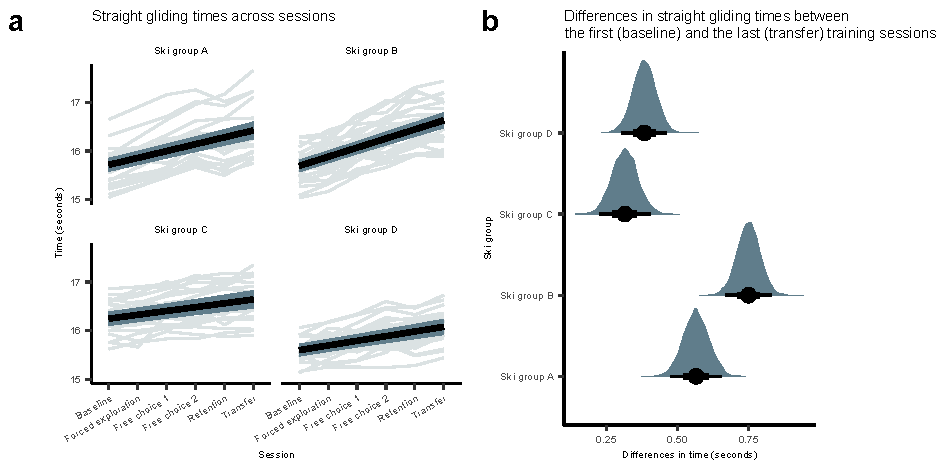
\includegraphics[width=1\linewidth]{figure/figure_methodological_straightgliding.pdf}
    \caption{Enter Caption}
    \label{fig:straightgliding}
\end{figure}